% ------------------------------------------------------------------------------
% TYPO3 Version 10.1 - What's New (Dutch Version)
%
% @license	Creative Commons BY-NC-SA 3.0
% @link		http://typo3.org/download/release-notes/whats-new/
% @language	Dutch
% ------------------------------------------------------------------------------

\section{Gebruikersinterface backend}
\begin{frame}[fragile]
	\frametitle{Gebruikersinterface backend}

	\begin{center}\huge{Hoofdstuk 1:}\end{center}
	\begin{center}\huge{\color{typo3darkgrey}\textbf{Gebruikersinterface backend}}\end{center}

\end{frame}

% ------------------------------------------------------------------------------
% Feature | 89115 | Auto slug update and redirect creation on slug change

\begin{frame}[fragile]
	\frametitle{Gebruikersinterface backend}
	\framesubtitle{Slug bijwerken en doorverwijzen (1)}

	\begin{itemize}
		\item Als backendgebruikers het URL-pad van een pagina (zgn "slug") aanpassen
			is de oude URL niet meer beschikbaar.
		\item Dit resulteert mogelijk in een "pagina niet gevonden" melding voor deze
			pagina, inclusief de URL's van alle subpagina's.
	\end{itemize}

	\begin{figure}
		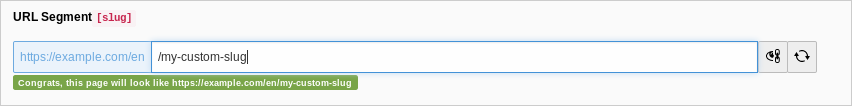
\includegraphics[width=0.80\linewidth]{BackendUserInterface/89115b-AutoSlugUpdateAndRedirectCreationOnSlugChange.png}
	\end{figure}

	\begin{itemize}
		\item Sinds TYPO3 v10.1, voorkomen twee acties dat dit gebeurt:

			\begin{itemize}
				\item slugs worden voor alle subpagina's automatisch bijgewerkt
				\item doorverwijzingen worden aangemaakt van de oude naar de nieuwe URL's
			\end{itemize}

	\end{itemize}

\end{frame}

% ------------------------------------------------------------------------------
% Feature | 89115 | Auto slug update and redirect creation on slug change

\begin{frame}[fragile]
	\frametitle{Gebruikersinterface backend}
	\framesubtitle{Slug bijwerken en doorverwijzen (2)}

	\begin{itemize}
		\item Backendgebruikers krijgen een melding over deze acties en ze kunnen
			ze eenvoudig terugdraaien met een enkele klik:

	\end{itemize}

	\begin{figure}
		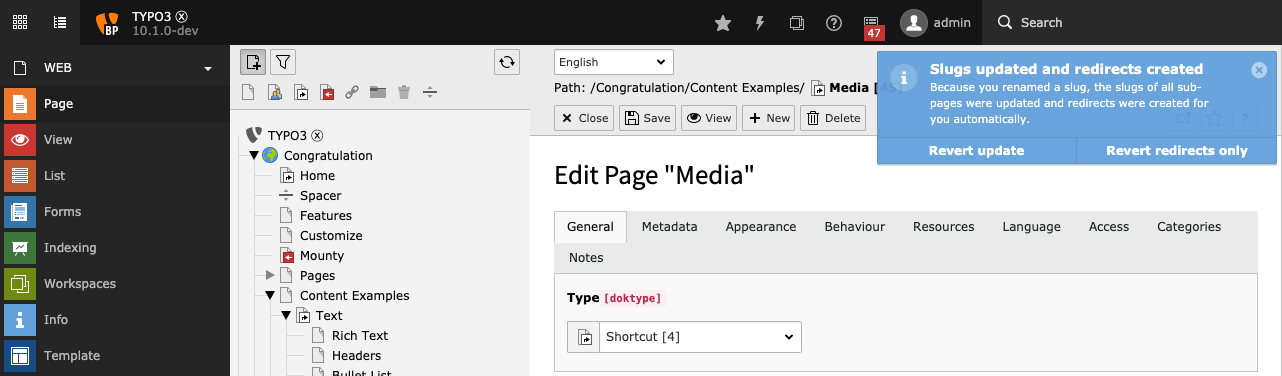
\includegraphics[width=0.80\linewidth]{BackendUserInterface/89115c-AutoSlugUpdateAndRedirectCreationOnSlugChange.png}
	\end{figure}

\end{frame}

% ------------------------------------------------------------------------------
% Feature | 85918 | Hide in menu / Show in menu entry for pages in context menu

\begin{frame}[fragile]
	\frametitle{Gebruikersinterface backend}
	\framesubtitle{Tonen/verbergen in menu}

	In het contextmenu zit een nieuwe optie om pagina's te tonen/verbergen.

	\begin{figure}
		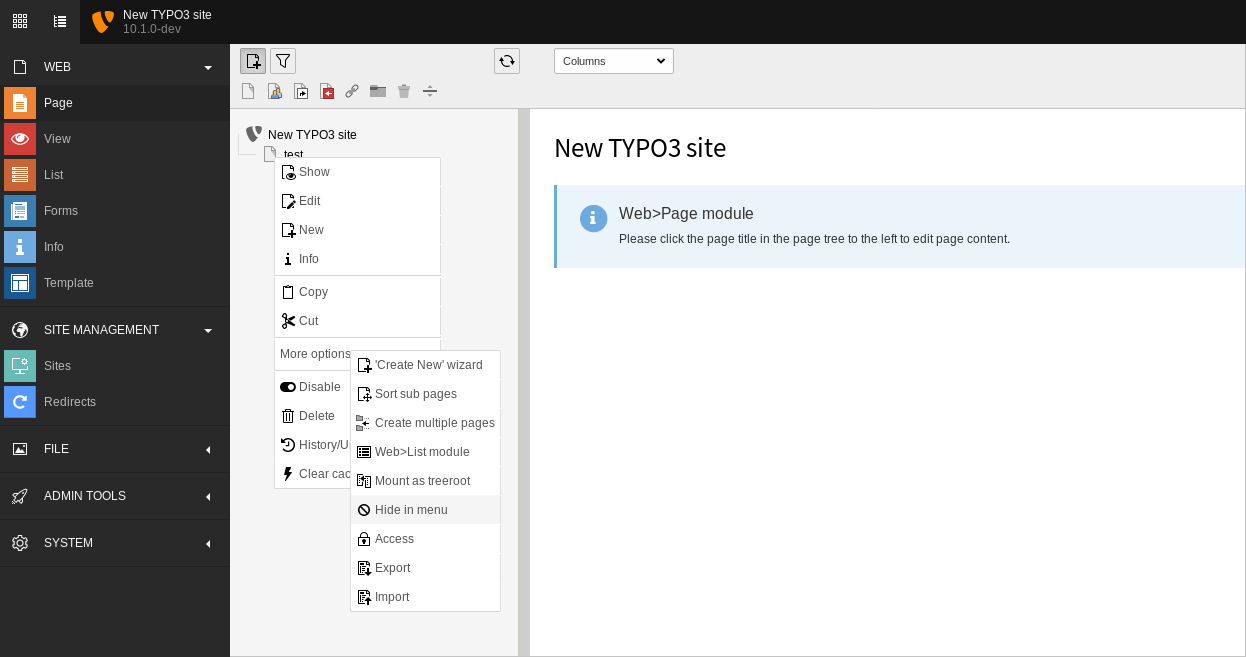
\includegraphics[width=0.80\linewidth]{BackendUserInterface/85918-HideShowInMenu-InContextMenu.png}
	\end{figure}

\end{frame}

% ------------------------------------------------------------------------------
